% Created by tikzDevice version 0.10.1 on 2020-02-15 16:05:40
% !TEX encoding = UTF-8 Unicode
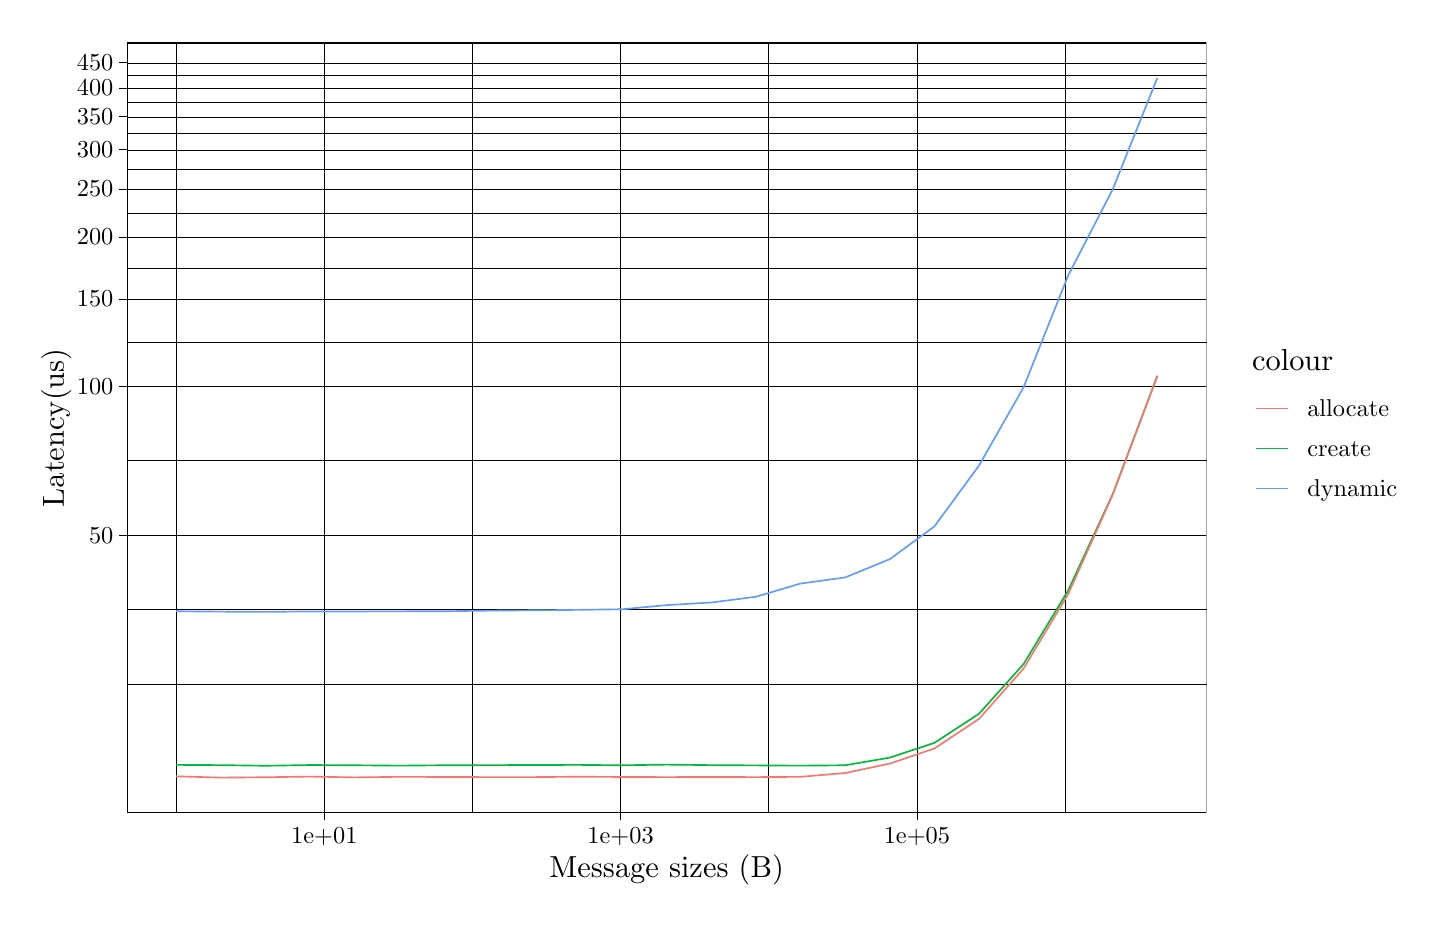
\begin{tikzpicture}[x=1pt,y=1pt]
\definecolor{fillColor}{RGB}{255,255,255}
\path[use as bounding box,fill=fillColor,fill opacity=0.00] (0,0) rectangle (505.89,314.37);
\begin{scope}
\path[clip] (  0.00,  0.00) rectangle (505.89,314.37);
\definecolor{drawColor}{RGB}{255,255,255}
\definecolor{fillColor}{RGB}{255,255,255}

\path[draw=drawColor,line width= 0.6pt,line join=round,line cap=round,fill=fillColor] (  0.00,  0.00) rectangle (505.89,314.37);
\end{scope}
\begin{scope}
\path[clip] ( 35.92, 30.72) rectangle (425.93,308.87);
\definecolor{fillColor}{RGB}{255,255,255}

\path[fill=fillColor] ( 35.92, 30.72) rectangle (425.93,308.87);
\definecolor{drawColor}{RGB}{0,0,0}

\path[draw=drawColor,line width= 0.0pt,line join=round] ( 35.92, 77.04) --
	(425.93, 77.04);

\path[draw=drawColor,line width= 0.0pt,line join=round] ( 35.92,103.98) --
	(425.93,103.98);

\path[draw=drawColor,line width= 0.0pt,line join=round] ( 35.92,157.86) --
	(425.93,157.86);

\path[draw=drawColor,line width= 0.0pt,line join=round] ( 35.92,200.56) --
	(425.93,200.56);

\path[draw=drawColor,line width= 0.0pt,line join=round] ( 35.92,227.50) --
	(425.93,227.50);

\path[draw=drawColor,line width= 0.0pt,line join=round] ( 35.92,247.35) --
	(425.93,247.35);

\path[draw=drawColor,line width= 0.0pt,line join=round] ( 35.92,263.11) --
	(425.93,263.11);

\path[draw=drawColor,line width= 0.0pt,line join=round] ( 35.92,276.19) --
	(425.93,276.19);

\path[draw=drawColor,line width= 0.0pt,line join=round] ( 35.92,287.37) --
	(425.93,287.37);

\path[draw=drawColor,line width= 0.0pt,line join=round] ( 35.92,297.14) --
	(425.93,297.14);

\path[draw=drawColor,line width= 0.0pt,line join=round] ( 53.64, 30.72) --
	( 53.64,308.87);

\path[draw=drawColor,line width= 0.0pt,line join=round] (160.72, 30.72) --
	(160.72,308.87);

\path[draw=drawColor,line width= 0.0pt,line join=round] (267.79, 30.72) --
	(267.79,308.87);

\path[draw=drawColor,line width= 0.0pt,line join=round] (374.87, 30.72) --
	(374.87,308.87);

\path[draw=drawColor,line width= 0.1pt,line join=round] ( 35.92,130.92) --
	(425.93,130.92);

\path[draw=drawColor,line width= 0.1pt,line join=round] ( 35.92,184.80) --
	(425.93,184.80);

\path[draw=drawColor,line width= 0.1pt,line join=round] ( 35.92,216.32) --
	(425.93,216.32);

\path[draw=drawColor,line width= 0.1pt,line join=round] ( 35.92,238.68) --
	(425.93,238.68);

\path[draw=drawColor,line width= 0.1pt,line join=round] ( 35.92,256.03) --
	(425.93,256.03);

\path[draw=drawColor,line width= 0.1pt,line join=round] ( 35.92,270.20) --
	(425.93,270.20);

\path[draw=drawColor,line width= 0.1pt,line join=round] ( 35.92,282.18) --
	(425.93,282.18);

\path[draw=drawColor,line width= 0.1pt,line join=round] ( 35.92,292.56) --
	(425.93,292.56);

\path[draw=drawColor,line width= 0.1pt,line join=round] ( 35.92,301.71) --
	(425.93,301.71);

\path[draw=drawColor,line width= 0.1pt,line join=round] (107.18, 30.72) --
	(107.18,308.87);

\path[draw=drawColor,line width= 0.1pt,line join=round] (214.26, 30.72) --
	(214.26,308.87);

\path[draw=drawColor,line width= 0.1pt,line join=round] (321.33, 30.72) --
	(321.33,308.87);
\definecolor{drawColor}{RGB}{0,186,56}

\path[draw=drawColor,line width= 0.6pt,line join=round] ( 53.64, 47.98) --
	( 69.76, 47.89) --
	( 85.88, 47.66) --
	(101.99, 47.93) --
	(118.11, 47.84) --
	(134.23, 47.70) --
	(150.34, 47.84) --
	(166.46, 47.89) --
	(182.58, 47.93) --
	(198.69, 47.98) --
	(214.81, 47.84) --
	(230.92, 48.07) --
	(247.04, 47.89) --
	(263.16, 47.79) --
	(279.27, 47.70) --
	(295.39, 47.84) --
	(311.51, 50.60) --
	(327.62, 55.92) --
	(343.74, 66.43) --
	(359.86, 84.40) --
	(375.97,110.99) --
	(392.09,145.83) --
	(408.20,188.58);
\definecolor{drawColor}{RGB}{248,118,109}

\path[draw=drawColor,line width= 0.6pt,line join=round] ( 53.64, 43.85) --
	( 69.76, 43.37) --
	( 85.88, 43.51) --
	(101.99, 43.75) --
	(118.11, 43.46) --
	(134.23, 43.66) --
	(150.34, 43.61) --
	(166.46, 43.56) --
	(182.58, 43.56) --
	(198.69, 43.70) --
	(214.81, 43.61) --
	(230.92, 43.56) --
	(247.04, 43.61) --
	(263.16, 43.56) --
	(279.27, 43.66) --
	(295.39, 45.03) --
	(311.51, 48.43) --
	(327.62, 53.89) --
	(343.74, 64.59) --
	(359.86, 82.80) --
	(375.97,109.65) --
	(392.09,145.66) --
	(408.20,188.48);
\definecolor{drawColor}{RGB}{97,156,255}

\path[draw=drawColor,line width= 0.6pt,line join=round] ( 53.64,103.49) --
	( 69.76,103.35) --
	( 85.88,103.27) --
	(101.99,103.42) --
	(118.11,103.42) --
	(134.23,103.46) --
	(150.34,103.49) --
	(166.46,103.71) --
	(182.58,103.84) --
	(198.69,103.99) --
	(214.81,104.21) --
	(230.92,105.71) --
	(247.04,106.65) --
	(263.16,108.73) --
	(279.27,113.50) --
	(295.39,115.71) --
	(311.51,122.30) --
	(327.62,134.12) --
	(343.74,156.11) --
	(359.86,184.39) --
	(375.97,224.81) --
	(392.09,255.98) --
	(408.20,296.23);
\definecolor{drawColor}{RGB}{0,0,0}

\path[draw=drawColor,line width= 0.6pt,line join=round,line cap=round] ( 35.92, 30.72) rectangle (425.93,308.87);
\end{scope}
\begin{scope}
\path[clip] (  0.00,  0.00) rectangle (505.89,314.37);
\definecolor{drawColor}{RGB}{0,0,0}

\node[text=drawColor,anchor=base west,inner sep=0pt, outer sep=0pt, scale=  0.88] at ( 22.17,128.10) {50};

\node[text=drawColor,anchor=base west,inner sep=0pt, outer sep=0pt, scale=  0.88] at ( 17.77,181.98) {100};

\node[text=drawColor,anchor=base west,inner sep=0pt, outer sep=0pt, scale=  0.88] at ( 17.77,213.50) {150};

\node[text=drawColor,anchor=base west,inner sep=0pt, outer sep=0pt, scale=  0.88] at ( 17.77,235.86) {200};

\node[text=drawColor,anchor=base west,inner sep=0pt, outer sep=0pt, scale=  0.88] at ( 17.77,253.20) {250};

\node[text=drawColor,anchor=base west,inner sep=0pt, outer sep=0pt, scale=  0.88] at ( 17.77,267.37) {300};

\node[text=drawColor,anchor=base west,inner sep=0pt, outer sep=0pt, scale=  0.88] at ( 17.77,279.36) {350};

\node[text=drawColor,anchor=base west,inner sep=0pt, outer sep=0pt, scale=  0.88] at ( 17.77,289.74) {400};

\node[text=drawColor,anchor=base west,inner sep=0pt, outer sep=0pt, scale=  0.88] at ( 17.77,298.89) {450};
\end{scope}
\begin{scope}
\path[clip] (  0.00,  0.00) rectangle (505.89,314.37);
\definecolor{drawColor}{RGB}{0,0,0}

\path[draw=drawColor,line width= 0.3pt,line join=round] ( 33.17,130.92) --
	( 35.92,130.92);

\path[draw=drawColor,line width= 0.3pt,line join=round] ( 33.17,184.80) --
	( 35.92,184.80);

\path[draw=drawColor,line width= 0.3pt,line join=round] ( 33.17,216.32) --
	( 35.92,216.32);

\path[draw=drawColor,line width= 0.3pt,line join=round] ( 33.17,238.68) --
	( 35.92,238.68);

\path[draw=drawColor,line width= 0.3pt,line join=round] ( 33.17,256.03) --
	( 35.92,256.03);

\path[draw=drawColor,line width= 0.3pt,line join=round] ( 33.17,270.20) --
	( 35.92,270.20);

\path[draw=drawColor,line width= 0.3pt,line join=round] ( 33.17,282.18) --
	( 35.92,282.18);

\path[draw=drawColor,line width= 0.3pt,line join=round] ( 33.17,292.56) --
	( 35.92,292.56);

\path[draw=drawColor,line width= 0.3pt,line join=round] ( 33.17,301.71) --
	( 35.92,301.71);
\end{scope}
\begin{scope}
\path[clip] (  0.00,  0.00) rectangle (505.89,314.37);
\definecolor{drawColor}{RGB}{0,0,0}

\path[draw=drawColor,line width= 0.3pt,line join=round] (107.18, 27.97) --
	(107.18, 30.72);

\path[draw=drawColor,line width= 0.3pt,line join=round] (214.26, 27.97) --
	(214.26, 30.72);

\path[draw=drawColor,line width= 0.3pt,line join=round] (321.33, 27.97) --
	(321.33, 30.72);
\end{scope}
\begin{scope}
\path[clip] (  0.00,  0.00) rectangle (505.89,314.37);
\definecolor{drawColor}{RGB}{0,0,0}

\node[text=drawColor,anchor=base,inner sep=0pt, outer sep=0pt, scale=  0.88] at (107.18, 19.71) {1e+01};

\node[text=drawColor,anchor=base,inner sep=0pt, outer sep=0pt, scale=  0.88] at (214.26, 19.71) {1e+03};

\node[text=drawColor,anchor=base,inner sep=0pt, outer sep=0pt, scale=  0.88] at (321.33, 19.71) {1e+05};
\end{scope}
\begin{scope}
\path[clip] (  0.00,  0.00) rectangle (505.89,314.37);
\definecolor{drawColor}{RGB}{0,0,0}

\node[text=drawColor,anchor=base,inner sep=0pt, outer sep=0pt, scale=  1.10] at (230.92,  7.44) {Message sizes (B)};
\end{scope}
\begin{scope}
\path[clip] (  0.00,  0.00) rectangle (505.89,314.37);
\definecolor{drawColor}{RGB}{0,0,0}

\node[text=drawColor,rotate= 90.00,anchor=base,inner sep=0pt, outer sep=0pt, scale=  1.10] at ( 13.08,169.80) {Latency(us)};
\end{scope}
\begin{scope}
\path[clip] (  0.00,  0.00) rectangle (505.89,314.37);
\definecolor{fillColor}{RGB}{255,255,255}

\path[fill=fillColor] (436.93,135.11) rectangle (500.39,204.49);
\end{scope}
\begin{scope}
\path[clip] (  0.00,  0.00) rectangle (505.89,314.37);
\definecolor{drawColor}{RGB}{0,0,0}

\node[text=drawColor,anchor=base west,inner sep=0pt, outer sep=0pt, scale=  1.10] at (442.43,190.44) {colour};
\end{scope}
\begin{scope}
\path[clip] (  0.00,  0.00) rectangle (505.89,314.37);
\definecolor{fillColor}{RGB}{255,255,255}

\path[fill=fillColor] (442.43,169.52) rectangle (456.89,183.97);
\end{scope}
\begin{scope}
\path[clip] (  0.00,  0.00) rectangle (505.89,314.37);
\definecolor{drawColor}{RGB}{248,118,109}

\path[draw=drawColor,line width= 0.6pt,line join=round] (443.88,176.74) -- (455.44,176.74);
\end{scope}
\begin{scope}
\path[clip] (  0.00,  0.00) rectangle (505.89,314.37);
\definecolor{drawColor}{RGB}{248,118,109}

\path[draw=drawColor,line width= 0.6pt,line join=round] (443.88,176.74) -- (455.44,176.74);
\end{scope}
\begin{scope}
\path[clip] (  0.00,  0.00) rectangle (505.89,314.37);
\definecolor{drawColor}{RGB}{248,118,109}

\path[draw=drawColor,line width= 0.6pt,line join=round] (443.88,176.74) -- (455.44,176.74);
\end{scope}
\begin{scope}
\path[clip] (  0.00,  0.00) rectangle (505.89,314.37);
\definecolor{fillColor}{RGB}{255,255,255}

\path[fill=fillColor] (442.43,155.06) rectangle (456.89,169.52);
\end{scope}
\begin{scope}
\path[clip] (  0.00,  0.00) rectangle (505.89,314.37);
\definecolor{drawColor}{RGB}{0,186,56}

\path[draw=drawColor,line width= 0.6pt,line join=round] (443.88,162.29) -- (455.44,162.29);
\end{scope}
\begin{scope}
\path[clip] (  0.00,  0.00) rectangle (505.89,314.37);
\definecolor{drawColor}{RGB}{0,186,56}

\path[draw=drawColor,line width= 0.6pt,line join=round] (443.88,162.29) -- (455.44,162.29);
\end{scope}
\begin{scope}
\path[clip] (  0.00,  0.00) rectangle (505.89,314.37);
\definecolor{drawColor}{RGB}{0,186,56}

\path[draw=drawColor,line width= 0.6pt,line join=round] (443.88,162.29) -- (455.44,162.29);
\end{scope}
\begin{scope}
\path[clip] (  0.00,  0.00) rectangle (505.89,314.37);
\definecolor{fillColor}{RGB}{255,255,255}

\path[fill=fillColor] (442.43,140.61) rectangle (456.89,155.06);
\end{scope}
\begin{scope}
\path[clip] (  0.00,  0.00) rectangle (505.89,314.37);
\definecolor{drawColor}{RGB}{97,156,255}

\path[draw=drawColor,line width= 0.6pt,line join=round] (443.88,147.84) -- (455.44,147.84);
\end{scope}
\begin{scope}
\path[clip] (  0.00,  0.00) rectangle (505.89,314.37);
\definecolor{drawColor}{RGB}{97,156,255}

\path[draw=drawColor,line width= 0.6pt,line join=round] (443.88,147.84) -- (455.44,147.84);
\end{scope}
\begin{scope}
\path[clip] (  0.00,  0.00) rectangle (505.89,314.37);
\definecolor{drawColor}{RGB}{97,156,255}

\path[draw=drawColor,line width= 0.6pt,line join=round] (443.88,147.84) -- (455.44,147.84);
\end{scope}
\begin{scope}
\path[clip] (  0.00,  0.00) rectangle (505.89,314.37);
\definecolor{drawColor}{RGB}{0,0,0}

\node[text=drawColor,anchor=base west,inner sep=0pt, outer sep=0pt, scale=  0.88] at (462.39,173.71) {allocate};
\end{scope}
\begin{scope}
\path[clip] (  0.00,  0.00) rectangle (505.89,314.37);
\definecolor{drawColor}{RGB}{0,0,0}

\node[text=drawColor,anchor=base west,inner sep=0pt, outer sep=0pt, scale=  0.88] at (462.39,159.26) {create};
\end{scope}
\begin{scope}
\path[clip] (  0.00,  0.00) rectangle (505.89,314.37);
\definecolor{drawColor}{RGB}{0,0,0}

\node[text=drawColor,anchor=base west,inner sep=0pt, outer sep=0pt, scale=  0.88] at (462.39,144.81) {dynamic};
\end{scope}
\end{tikzpicture}
